\section{Introduction}
In the previous chapter we reported strong evidence for a normal mode that exists purely on the hinge or side of \ac{FTS}. To verify that the observed mode does not come from the bulk or c-axis of the material we draped a thick, insulating material over the \ac{FTS} flake that acts as a control tunneling interface. Here we extend that work . Most notably, the physics that leads to a hinge mode in \ac{FTS} also predicts that the normal mode should have a linear dispersion and thus the tunneling conductance should have a flat plateau below the superconducting gap energy\cite{Zhang2019}. The fabrication steps required to place an insulating \ac{hBN} flake over the hinge of the material also causes the exposed hinges to come into contact with polymers at temperatures over 90 centigrade. 

\section{Observation of Bias-Independent Conductance Plateau}
The most striking feature of the resultant $\frac{dI}{dV}$ vs $v_{bias}$ is the bias-independent conductance plateau shown in Fig \ref{fig:PARDeviceFab}. The behavior of this plateau with respect to energy, conductance, and temperature all indicate that \ac{PAR} is occurring at the interface. More specifically, after the spectra is properly normalized using the self-consistent method demonstrated by Chen T. Y., \textit{et al.} \cite{Chen2010} the sub-gap conductance is exactly twice the normal state conductance. Furthermore, this plateau extends out to 4.6 meV which is consistent with gaps sizes measure using similar methods\cite{Tang2019}. However a key difference between this spectrum and the \ac{PAR} spectra expected from a standard s-wave superconductor is the rate at which the conductance saturates with temperature. In the calculated \ac{BTK} spectrum, the zero-bias conductance does not saturate at twice the background conductance until around $0.1T_{c}$ whereas the observed \ac{PAR} in \ac{FTS} saturates much quicker at $0.9T_{c}$. 
\begin{figure}
    \centering
    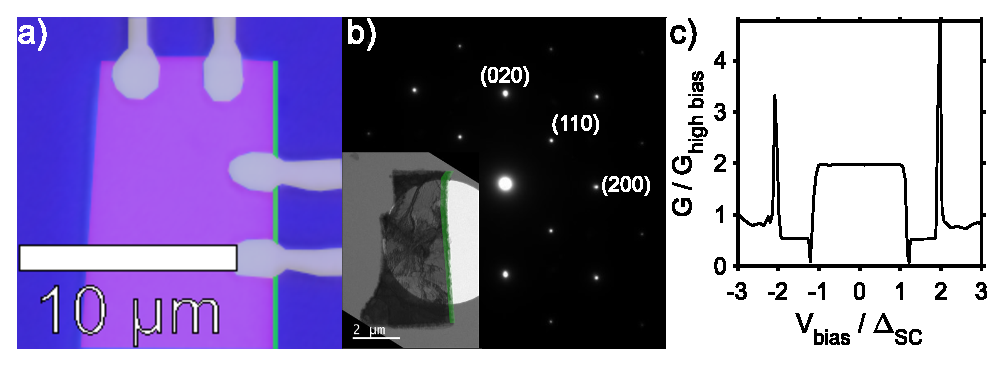
\includegraphics[width = \textwidth]{Chap4/Figures/DeviceFab.eps}
    \caption{a) False color optical image of a representative device with a straight (100) edge which is highlighted in green. b) \ac{TEM} diffraction pattern demonstrating the (100) edge. Inset shows the flake measured as well as the diffraction aperture. c) Base temperature differential conductance curve.}
    \label{fig:PARDeviceFab}
\end{figure}
\begin{figure}
    \centering
    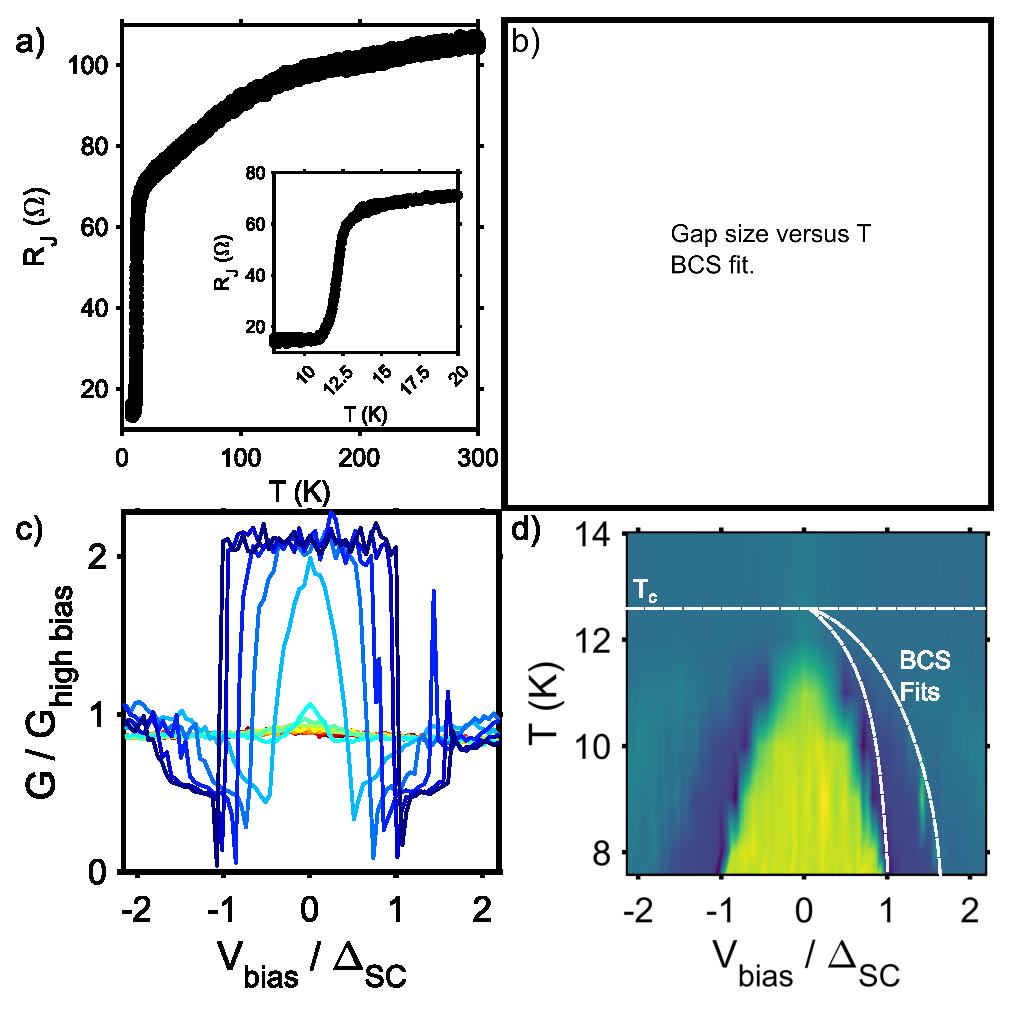
\includegraphics[width = \textwidth]{Chap4/Figures/Temperature.eps}
    \caption{Caption}
    \label{fig:PARTemp}
\end{figure}
\section{Magnetic Field Dependence}
\begin{figure}
    \centering
    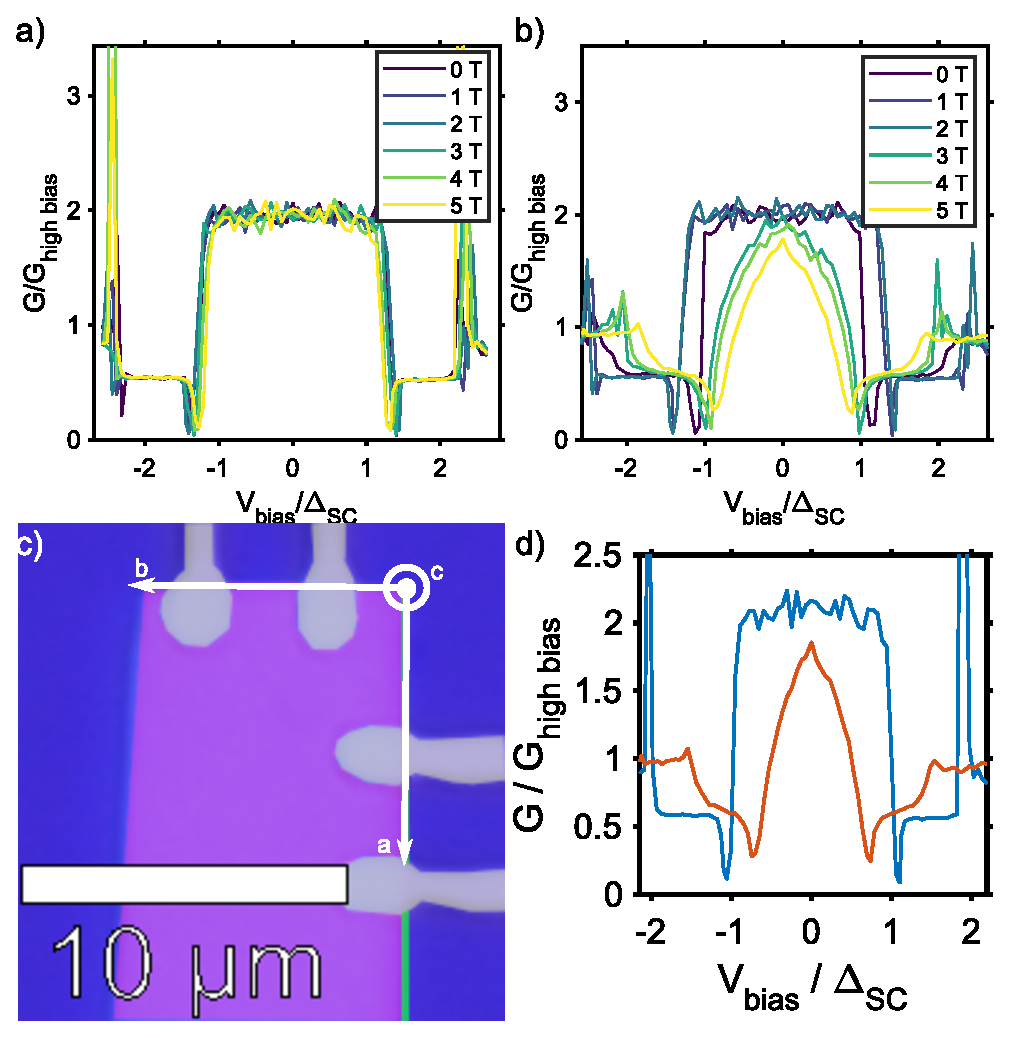
\includegraphics[width = \textwidth]{Chap4/Figures/MagneticField.eps}
    \caption{Caption}
    \label{fig:PARField}
\end{figure}
\section{Conclusion}